\chapter{¿Es exacto el filtro?}
\label{cap:nuts}

La actualización de Laplace reemplaza cada posterior por una gaussiana. La aproximación puede fallar de dos maneras: la posterior de un partido no es gaussiana (los goles son pocos y discretos), y los errores se acumulan a lo largo de cientos de actualizaciones. La pregunta se puede responder directamente, porque en una ventana corta la posterior exacta es calculable.

\section{Diseño}

La prueba se hizo con el núcleo, cuya posterior es más fácil de escribir en NumPyro; el modelo oficial usa la misma actualización con un Newton en cuatro dimensiones en vez de dos. Se toma el estado del filtro al comienzo de la Premier 2025-26 como prior gaussiano. Sobre él se escribe el modelo completo de la media temporada siguiente: el estado semanal con paseo aleatorio y los mismos hiperparámetros, y la verosimilitud de Dixon–Coles de los 191 partidos jugados en esas 21 semanas. Esa posterior se muestrea con NUTS~\cite{hoffman2014} en NumPyro~\cite{numpyro2019}. Al final de la ventana, la posterior suavizada en el último instante coincide con la posterior de filtrado, así que la comparación con el filtro es directa: medias y desviaciones de la fuerza neta de cada equipo y, simulando la segunda mitad con cada una, la matriz de posiciones finales (\code{scripts/nuts\_validation.py}).

\section{Resultados}

\begin{figure}[h]
\centering
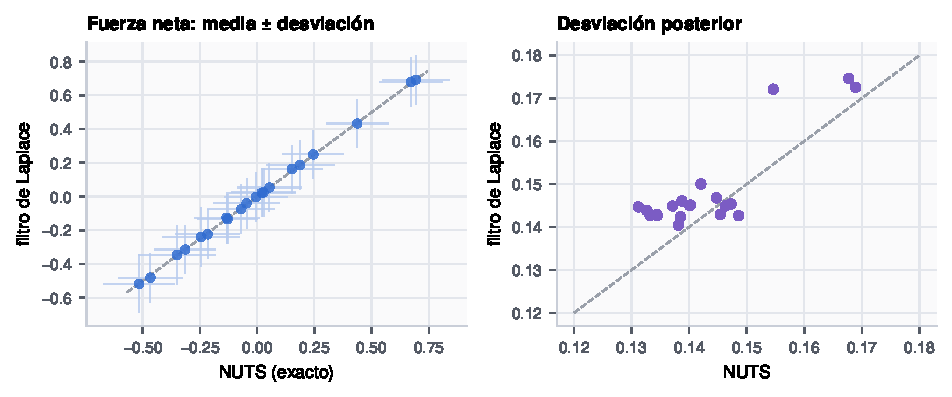
\includegraphics[width=\textwidth]{nuts}
\caption{Fuerza neta de los 20 equipos de la Premier 2025-26 a mitad de temporada, con la posterior exacta (NUTS) y con el filtro de Laplace. Izquierda: medias con barras de una desviación. Derecha: desviaciones posteriores.}
\label{fig:nuts}
\end{figure}

La tabla~\ref{tab:nuts} resume la comparación (R3). Las medias coinciden casi exactamente y las desviaciones del filtro son en promedio un 4\,\% más chicas que las exactas. La distancia de variación total entre las distribuciones de posición final, promediada sobre los equipos, es $0{,}022$, del orden del ruido de Monte Carlo de las simulaciones con que se compara. NUTS no registró divergencias.

\begin{table}[h]
\centering
\caption{Filtro de Laplace frente a NUTS, Premier 2025-26 a mitad de temporada (R3).}
\label{tab:nuts}
\small
\begin{tabular}{@{}lr@{}}
\toprule
\hd{Medida} & \hd{Valor} \\
\midrule
Correlación de las medias de la fuerza neta & $0{,}9999$ \\
Máxima diferencia de medias & $0{,}015$ \\
Razón de desviaciones (filtro / exacto), promedio & $0{,}96$ \\
Variación total en la posición final, promedio y máximo & $0{,}022$; $0{,}042$ \\
Divergencias de NUTS & 0 \\
\bottomrule
\end{tabular}
\end{table}

La conclusión es que la aproximación gaussiana no es el cuello de botella del modelo. Una media temporada aporta más de diez partidos por equipo y la posterior de las fuerzas es casi gaussiana. Lo que sí importa es propagar la covarianza completa del filtro a la simulación, que es el tema del capítulo~\ref{cap:sim}.

\begin{nota}{Lo que el filtro no hace}
El filtro no vuelve atrás: la fuerza de un equipo en septiembre no se corrige con lo que se aprende en marzo. Para pronosticar no hace falta, porque solo interesa el estado de hoy, y el paseo aleatorio garantiza que la creencia filtrada sobre hoy es la correcta dada toda la historia. Para describir la historia (``¿qué tan bueno era este equipo en septiembre?'') haría falta un suavizador de Rauch–Tung–Striebel, que no se implementó.
\end{nota}
